%!TEX root = ../fbi.tex

\section{Conclusion and Discussion}

\appendix

\section{Determining the edge action of the symmetry using MPS}
\label{Appendix:MPS}

We can use the formalism of MPS to assign an action
of the symmetry on the Schmidt states, and in particular for the charge and 
translation on-site symmetries the Schmidt states can be simultaneously assigned
charge and translation quantum numbers. This method of discovering the symmetry 
action will reproduce the action discussed in \ref{sec:ES} and quantum numbers used
in the spectra plots shown in Fig.~\ref{fig:ESL910}.
  
Let's discuss this formalism briefly. In addition,
we will discuss a generalization of this method that allows us to numerically
determine the symmetry action of inversion symmetry on the Schmidt states,
as in Section~\ref{sec:symmetry}. 
Both of these discussions follow Ref.~\onlinecite{pollmann2010}.

These discussions start by finding tensors $\Gamma, \Lambda$ representing the 
so-called canonical form of the MPS, as
originally detailed in \cite{perezgarcia2008}. This canonical form provides the Schmidt
decomposition at each site in the lattice.
\beq
\ket{\psi} = \sum\limits_{\{p_i\}} \ldots \Lambda \Gamma_{p_0} \Lambda \Gamma_{p_1} \Lambda \Gamma_{p_2} \Lambda \ldots \ket{... p_0 p_1 p_2 ...}.
\eeq
As a reminder, each physical leg represents all $2W$ physical sites on a cylinder slice,
and each virtual leg represents all virtual indices that connect cylinder slices.
The change of basis to canonical form generally mixes the Hilbert spaces from these
virtual legs, so the resulting basis won't be local around the circumference
of the cylinder.

Each on-site symmetry of the wavefunction $U_g = \otimes_i u^i_g$, with $U_g
\ket{\psi} = e^{i \Theta_g} \ket{\psi}$ is assigned an operator $V_g$ that
acts on the virtual leg of the MPS, that satisfies the equation
\begin{center}
\beq
\label{eq:onsitesym}
\eeq
\vskip-5em
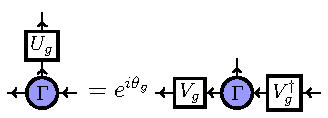
\includegraphics[width=0.6\columnwidth]{group_sym.pdf}.
\end{center}
This equation can be rewritten and solved as an eigenvector problem;
for an MPS with a nondegenerate largest transfer matrix eigenvalue,
this equation is guaranteed have a unique solution where the eigenvalue $e^{i \theta_g}$
is the largest eigenvalue of the eigenvector problem.

The solutions $V_g$ have two important properties: they are only defined up to a phase,
and they are guaranteed to commute with the diagonal matrix $\Lambda$ of Schmidt weights.  

Due to the first property, these operators are not guaranteed to form a linear
representation of the group of on-site symmetries, but in general could make
up a projective representation, satisfying
$$V_g V_h = e^{i \omega(g, h)} V_{gh}.$$ 
It is not always possible to absorb these phases into the definitions of the $V_g$.
The set of equivalent classes of phases $\omega(g, h)$ 
under redefinitions $V_g \to \alpha(g)V_g$ is called $H^2(G, U(1))$, the second group 
cohomology with $U(1)$ coefficients. 

For all the groups discussed in this paper, the group cohomology classes are labeled by
elements of a discrete abelian group - these discrete classes cannot be connected to each other
continuously. Physically, only a phase transition or breaking the symmetry allows one to connect
the different projective symmetry actions. 
Additionally, the classification of projective representations for the on-site symmetry group 
$U(1) \times \mathbb{Z}_W$ representing charge and translation around the cylinder is trivial. 
Thus, these edge symmetries can be taken to act linearly, 
and all Schmidt states can always be simultaneously assigned charge and momentum eigenvalues,
as in Figure~\ref{fig:ESL910}.

The second property guarantees that the $V_g$ only mixes exactly degenerate Schmidt states.
The action of $V_g$ must have the same phases $\omega(g, h)$ on each degenerate block of Schmidt 
states, so the projective representation can be nontrivial on any block only if every Schmidt 
state throughout the entire spectrum is degenerate. The degeneracy will be protected by the 
symmetry if and only if the $V_g$ form a nontrivial projective representation. Therefore
this 1D SPT analysis can only potentially give a nontrival answer for the odd $W$ states 
of the HFBI, where this exact degeneracy is seen throughout the spectrum. Nonetheless, we find 
there are no on-site symmetries of the wavefunction that can be used to explain the degenerate
entanglement spectrum of the odd $W$ HFBI states. Instead we must use an inversion symmetry. 

The MPS analysis of inversion symmetry works similarly. We will consider in general any symmetry  
$h$ of the wavefunction that squares to the identity and that can be written in the MPS as the 
product of an on-site symmetry action $U_h$ and a transpose of the site tensor.
This will include an inversion of the honeycomb lattice - equivalent to a 180 degree rotation 
about the center of any plaquette, which we label $\I = \I_y \I_x$, and the combination of
inversion with on-site symmetries. In addition, by blocking two site-tensors together, we
can write the reflection symmetry $\I_y$ in this form as well. In this scenario, the 
edge symmetry action satisfies
\begin{center}
\beq
\label{eq:onsitesym}
\eeq
\vskip-5em
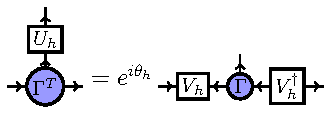
\includegraphics[width=0.6\columnwidth]{inv_sym.pdf}.
\end{center}
The map $V_{h}$ is also computed as a dominant eigenvector. 

For the HFBI, the symmetry group respected by the cylinder geometry is
$U(1) \times (\mathbb{Z}_W \rtimes \mathbb{Z}_2)
\times \mathbb{Z}_2^P \times \mathbb{Z}_2^T$, where the factors refer to charge
symmetry, translation around the cylinder, $\I_x$, $\I_y$, and $\tau$ respectively.
The $P$ and $T$ denote space-reversing and time-reversing symmetries, and signify the 
antiunitary action on the Schmidt states. 
%Compute the cohomology class of 
%$H^2(U(1) \times (\mathbb{Z}_W \rtimes \mathbb{Z}_2)
%\times \mathbb{Z}_2^P \times \mathbb{Z}_2^T ; U(1)) ?$
Many of the non-trivial projective
representations of such a complicated group will remain projective when the symmetry is
restricted to a subgroup - in this case, the full symmetry is not needed to protect the 
entanglement degeneracy. As shown in Table~\ref{table:sym}, the projective representation 
corresponding to the HFBI state can indeed be protected by any one of a number of subgroups 
of the full symmetry group, all involving inversions and charge parity.

The symmetry actions - both on-site and inversion symmetries -
are computed in the Schmidt basis, but can be transformed
into the basis $\vket{\{\sigma_i\}}$ determined by the virtual legs of the PEPS in
Figure~\ref{fig:FBI_PEPS_2}. 
In this case, the symmetry action $V_{\I_y}$ is precisely
a particle-hole symmetry in the local PEPS basis, with coefficients
$$
V_{\I_y}\vket{\sigma_1, \ldots, \sigma_{W}} = \vket{1-\sigma_1, \ldots, 1-\sigma_{W}}, 
$$
since a state where the $i^{th}$ hexagon contributes $\sigma_i$ bosons on the right is paired with
a state where the $i^{th}$ hexagon contributes $1-\sigma_i$ on the left.
Thus 
$$
V_{\I_y} = \prod\limits_i \sigma_i^x K,
$$
where K is complex conjugation in the local PEPS basis, and $\sigma_i^x$ is the Pauli
operator acting on the $i^{th}$ site of the local PEPS basis.

Charge symmetry acts locally as well:
$$
e^{i \theta \mathcal{Q}}\vket{\sigma_1, \ldots, \sigma_{W}} = e^{i \theta \sum(\sigma_i-1/2)}\vket{\sigma_1, \ldots, \sigma_{W}}.
$$
In particular, charge parity $V_{\varPi} = e^{i \theta \mathcal{Q}}$ can be written as
$$V_{\varPi} = e^{i \pi \sum(\sigma_i - 1/2)} = \prod\limits_i \sigma_i^z.$$

The combined action of charge parity and reflection across the cut takes the form 
$$
V_{\varPi \I_y} = \prod\limits_i \left(i \sigma_i^y \right) K,
$$
which is precisely the form that time-reversal acting on an ordinary spin-$\frac12$ chain takes.
When the circumference of the cylinder $W$ is odd, we see that
$$V_{\varPi \I_y}V_{\varPi \I_y}^{*} = -I.$$ 
The degeneracy of the entanglement spectrum can be seen as an application of Kramer's theorem.
Formally, this property is said to characterize the nontrivial projective representation
$$
H^2(\mathbb{Z}_2^P; U(1)) = \mathbb{Z}_2,
$$
and remains true while $\varPi \I_y$ is a symmetry and no phase transitions have occurred.

Time reversal symmetry acts as complex conjugation in the local PEPS basis $V_{\tau}=K$.
Translation and $\I_x$ act as permutations of the local PEPS basis:
\begin{equation*}
\begin{split}
V_{T}\vket{\sigma_1, \ldots, \sigma_{W}} &= \vket{\sigma_2, \ldots, \sigma_{W}, \sigma_{1}} \\
V_{\I_x}\vket{\sigma_1, \ldots, \sigma_{W}} &= \vket{\sigma_W, \ldots, \sigma_{1}}.
\end{split}
\end{equation*}
These symmetries can be combined with $V_{\varPi \I_y}$ to create the additional topological 
invariants shown in Table~\ref{table:sym}. A non-trivial projective 
representation in $$H^2(\mathbb{Z}_2 \times \mathbb{Z}_2; U(1)) = \mathbb{Z}_2$$
is created whenever two unitary symmetries that commute in the bulk satisfy 
$$V_{g_1} V_{g_2} V_{g_1}^{-1} V_{g_2}^{-1} = -I.$$
Each new invariant is related to a new set of pertubations that can't break the entanglement 
degeneracy. 

\section{Local Hamiltonian for the Edge free boson CFT}
\label{Appendix:LocalEdge}

B

\section{Mode expansion and symmetry action of free-boson CFT}
\label{Appendix:CFT}
How do the symmetry protecting operations act on the CFT states
$\ket{e, m, \{n_i\}, \{\bar{n}_i\}}$?

From that, infer how they act on the free boson fields $\phi$ and $\theta$.

Which perturbations to the CFT gap it out completely or spontaneously break the symmetry?

Are those pertubations forbidden by the implementation of symmetry on the edge.

\section{Variants on the HFBI wavefunction}
\subsection{Tuning soft-core bosons to hard-core}
In Equations~\eqref{eqn:Dsc} and \eqref{eqn:Dhc}, the tensor $D$ can be replaced by a more general form 
\begin{equation} \label{eqn:Dgen}
D_{p, i_0 i_1 i_2}  = \left\{ \begin{array}{ll}
													d_p  &: p =i_0+i_1+i_2  \\
													0  &:  \text{else}
													\end{array}
											\right. ,
\end{equation}
which the coefficients $d_p = 1,\, 1,\, \sqrt{2},\,\sqrt{6}$ for $p = 0,\, 1,\, 2,\, 3$ in the soft-core state and $d_p = 1,\, 1,\, 0,\, 0$ for $p = 0,\, 1,\, 2,\, 3$ in the hard-core state. We can continously tune the coefficients $d_2$ and $d_3$ from the soft-core to the hard-core values.
Upon doing so, we find that the transfer matrix spectrum remains gapped, with the correlation length monotonically increasing from the soft-core state to the hard-core state. 
Furthermore, the low energy parts of the entanglement spectrum do not change significantly through this tuning.
Therefore we expect that the hard-core and soft-core phases can be adiabatically connected with a 
path of local Hamiltonians, and all SPT results that apply to one state apply to the other. By choosing appropriate values of $d_2$ and $d_3$, we can also make replace the vacuum $\ket{0}$ in
Equation~\eqref{eq:def} with a constant background of $N$ filled bosons $\ket{N}$, or even make
states of spins $S$ where Equation~\eqref{eq:def} becomes
\begin{equation} \label{eq:spindef}
\ket{\psi} = \prod\limits_{\varhexagon} \left( \sum\limits_{i \in \varhexagon} S^{+}_{i} \right) \ket{S_z = m}.
\end{equation}

\subsection{Inversion Protected Phase}
Additionally, the tensor $W$ in Equation~\eqref{eq:W} can be replaced by the more general form
\begin{equation} \label{eq:Wgen}
W^{n_1 \ldots n_6}  = \left\{ \begin{array}{lr}
													p_x  : & n_x=1,\, n_y = 0
													\; \forall \; y \neq x \\
													0  : & \text{else}
													\end{array} \right.,
\end{equation}
which corresponds to modifying Equation~\eqref{eq:def} to 
\begin{equation} \label{eq:pdef}
\ket{\psi_{\ell}} = \prod\limits_{\varhexagon} \left( \sum\limits_{i \in \varhexagon} p_i b^{\dagger}_{i} \right) \ket{0}.
\end{equation}

This does not in general preserve the rotational symmetry of the state, but it does if the 
coefficients $p_0, \ldots p_5$ are in an angular momentum mode $$p_x = e^{i x \ell}$$ where
$\ell \in \{0, 2\pi/6, \ldots 5\pi/6 \}$. These 6 discrete solutions can't be continously tuned to one another while preserving all the lattice symmetries.

The state $\ket{\psi_{\ell=\pi}}$ can be shown to be related to state $\ket{\psi_{\ell=0}}$ discussed in the main text by a on-site unitary operator $U(\pi)$, 
where 
\begin{equation} \label{eq:Uphi}
U(\varphi) = \prod\limits_{j \in B} e^{i \varphi \hat{Q}_j}.
\end{equation}
Due to this relation, $\ket{\psi_{\ell=\pi}}$ and $\ket{\psi_{\ell=0}}$ have identical correlation lengths and entanglement spectra. 
However, the protecting symmetries from Table~\ref{table:sym} are mapped using conjugation
by $U(\pi)$ into a new set of protecting symmetries, shown in Table~\ref{table:pisym}. 

\begin{table}
\begin{tabular*}{\columnwidth}{@{\extracolsep{\stretch{1}}}*{4}{r}@{}}
\toprule
Group & Generators & Invariant & $i$  \\
\midrule
$\mathbb{Z}_2^P$ & $\{\I \}$ 
& $V_{\I} V_{\I}^* = -I$ &$-$ \\
$\mathbb{Z}_2^P$ & $\{\I_y \}$ 
&$V_{\I_y} V_{\I_y}^* = -I$ &$-$ \\ \hline
$\mathbb{Z}_2 \times \mathbb{Z}_2^{PT}$& $\{\varPi, \tau \varPi \I\}$ 
&$V_{\varPi} V_{\tau \varPi \I} V_{\varPi}^{-1} V_{\tau \varPi \I}^{-1} = -I$ &$+$ \\
$\mathbb{Z}_2 \times \mathbb{Z}_2^{PT}$& $\{\varPi, \tau \varPi \I_y\}$
&$V_{\varPi} V_{\tau \varPi \I_y} V_{\varPi}^{-1} V_{\tau \varPi \I_y}^{-1} = -I$ &$+$ \\
$\mathbb{Z}_2 \times \mathbb{Z}_2^{PT}$& $\{\varPi \I_x, \tau \varPi \I\}$
&$V_{\varPi \I_x} V_{\tau \varPi \I} V_{\varPi \I_x}^{-1} V_{\tau \varPi \I}^{-1} = -I$&$+$ \\
$\mathbb{Z}_2 \times \mathbb{Z}_2^{PT}$& $\{\varPi \I_x, \tau \varPi \I_y\}$
&$V_{\varPi \I_x} V_{\tau \varPi \I_y} V_{\varPi \I_x}^{-1} V_{\tau \varPi \I_y}^{-1} = -I$ &$+$\\
\bottomrule
\end{tabular*}
\caption{Summary of symmetry protecting invariants found for the $\ket{\psi_{\ell=\pi}}$ state. 
The degenerate entanglement spectrum cannot be split unless all 6 of the  minimal protecting symmetry groups are broken. }
\label{table:pisym}
\end{table}

Notably,
since
$$
U(\pi) \varPi \I U(\pi)^{\dagger} = \I, 
$$
this state has doubly degenerate entanglement spectra on odd cylinder sizes protected by lattice inversion symmetry alone.

A similar mapping for 1-D inversion protected states is discussed in Appendix A of Ref.~\onlinecite{pollmann2010}. As discussed \brayden{somewhere}, the state $\ket{\psi_{\ell=0}}$
on the $W=1$ cylinder is adiabatically connected to the 1-D Haldane insulator state discussed in
Ref.~\onlinecite{pollmann2010}. The new $\ket{\psi_{\ell=\pi}}$ state on the $W=1$ cylinder is instead adiabatically connected to the 1-D AKLT state. 

\label{Appendix:Variants}